\documentclass[a4paper,12pt]{article}

%%%%%%%%%%%%%%%%%%%%%%%%%%%%%%%%%%%%%%%%%%%%%%%%%%%%%%%%%%%%%%%%%%%%%%%%%%%%%%%%%%
%%%%%%%%%%%Hier wird das Seitenlayout festgelegt %%%%%%%%%%%%%%%%%%%%%%%%%%%%%%%%%
%%%%%%%%%%%%%%%%%%%%%%%%%%%%%%%%%%%%%%%%%%%%%%%%%%%%%%%%%%%%%%%%%%%%%%%%%%%%%%%%%%
\usepackage[
  %showframe,% Seitenlayout anzeigen
  left=2cm,
  right=2cm,
  top=3cm,
  bottom=3cm,
]{geometry}
%%%%%%%%%%%%%%%%%%%%%%%%%%%%%%%%%%%%%%%%%%%%%%%%%%%%%%%%%%%%%%%%%%%%%%%%%%%%%%%%%%
%%%%%%%%%%%Mit dem folgenden Paket/Befehl wir die Matheumgebung "align*"%%%%%%%%%%
%%%%%%%%%%%automatisch auf der nächsten Seite fortgesetzt, wenn diese länger%%%%%%
%%%%%%%%%%%als die aktuelle Seite geht%%%%%%%%%%%%%%%%%%%%%%%%%%%%%%%%%%%%%%%%%%%%
%%%%%%%%%%%%%%%%%%%%%%%%%%%%%%%%%%%%%%%%%%%%%%%%%%%%%%%%%%%%%%%%%%%%%%%%%%%%%%%%%%
\usepackage{autobreak}
\allowdisplaybreaks
%%%%%%%%%%%%%%%%%%%%%%%%%%%%%%%%%%%%%%%%%%%%%%%%%%%%%%%%%%%%%%%%%%%%%%%%%%%%%%%%%%
%%%%%%%%%%%Hier werden nützliche Zusatzpakete importiert %%%%%%%%%%%%%%%%%%%%%%%%%
%%%%%%%%%%%%%%%%%%%%%%%%%%%%%%%%%%%%%%%%%%%%%%%%%%%%%%%%%%%%%%%%%%%%%%%%%%%%%%%%%%
%\usepackage{fancyhdr}
\usepackage[ngerman,german]{babel}
\usepackage[utf8]{inputenc}
%\usepackage[latin1]{inputenc} % für Linux Nutzer
\usepackage{amsmath}
\usepackage{amssymb}
\usepackage{amsthm}
\usepackage{amsfonts}
\usepackage{extarrows}
\usepackage{enumerate}
\usepackage{enumitem}
%%%%%%%%%%%%%%%%%%%%%%%%%%%%%%%%%%%%%%%%%%%%%%%%%%%%%%%%%%%%%%%%%%%%%%%%%%%%%%%%%%%%
%%%%%%%%%%%Weitere Zeichenpakete für zusätzliche Symbole %%%%%%%%%%%%%%%%%%%%%%%%%%%
%%%%%%%%%%%%%%%%%%%%%%%%%%%%%%%%%%%%%%%%%%%%%%%%%%%%%%%%%%%%%%%%%%%%%%%%%%%%%%%%%%%%
\usepackage{stmaryrd}
\usepackage{wasysym}
\usepackage{pifont}
%%%%%%%%%%%%%%%%%%%%%%%%%%%%%%%%%%%%%%%%%%%%%%%%%%%%%%%%%%%%%%%%%%%%%%%%%%%%%%%%%%%%
%Mit dem folgenden Paket können einfache Rechnungen automatisch ausgerechnet werden%
%%%%%%%%%%%%%%%%%%%%%%%%%%%%%%%%%%%%%%%%%%%%%%%%%%%%%%%%%%%%%%%%%%%%%%%%%%%%%%%%%%%%
\usepackage{xfp}%Beispiel: \fpeval{3+5+6} => 14
\usepackage{fp}
\usepackage{spreadtab}%Tabellenberechnungen
\usepackage{tabularx}

\usepackage{graphicx}
\usepackage{tikz}
\usepackage{pgf}
\usepackage{hyperref}
\usepackage{xcolor}
\usepackage{color, colortbl}


%%%%%%%%%%%%%%%%%%%%%%%%%%%%%%%%%%%%%%%%%%%%%%%%%%%%%%%%%%%%%
%%%%%%%%%%%%%% Ganz viele Befehle %%%%%%%%%%%%%%%%%%%%%%%%%%%
%%%%%%%%%%%%%%%%%%%%%%%%%%%%%%%%%%%%%%%%%%%%%%%%%%%%%%%%%%%%%

% Mengen

\newcommand{\N}{\mathbb N}
\newcommand{\R}{\mathbb R}
\newcommand{\C}{\mathbb C}
\newcommand{\Z}{\mathbb Z}
\newcommand{\Q}{\mathbb Q}
\newcommand{\K}{\mathbb K}	

% Ableitungen

\newcommand{\pfrac}[1]{{\frac\partial{\partial #1}}}	% partielle Ableitung als Bruch, Argument ist Variable, nach der abgeleitet wird

% Griechische Buchstaben

\renewcommand{\phi}{\varphi}
\newcommand{\eps}{\varepsilon}

% Pfeile / Äquivalenzen 

\newcommand{\Ra}{\Rightarrow}							% "daraus folgt"
\newcommand{\ra}{\rightarrow}							% "daraus folgt"
\newcommand{\La}{\Leftarrow}							% (analog wie oben)
\newcommand{\la}{\leftarrow}							% (analog wie oben)
\newcommand{\eq}{\Leftrightarrow}						% äquivalent
\newcommand{\upto}{\nearrow}							% Konvergenz von unten
\newcommand{\downto}{\searrow}							% Konvergenz von oben

% Vektorräume

\newcommand{\inv}{{-1}}									% zum schnelleren Invertieren per ^\inv

\newcommand{\mat}[4]{\begin{pmatrix}#1&#2\\#3&#4\end{pmatrix}}
														% 2x2-Matrix
\newcommand{\vek}[2]{\begin{pmatrix}#1\\#2\end{pmatrix}}% 2dim. Vektor

\newcommand{\bpm}{\begin{pmatrix}}						% Matrix (Anfang)
\newcommand{\epm}{\end{pmatrix}}						% Matrix (Ende)

%%%%%%%%%%check und uncheck%%%%%%%%%%%%%%%%
\newcommand{\cmark}{\text{\ding{51}}}                   % Check-Mark
\newcommand{\xmark}{\text{\ding{55}}}                   % UncheckMark
	
\usepackage{polynom}
\usepackage{pdfpages}
%%%%%%%%%%%%%%%%%%%%%%%%%%%%%%%%%%%%%%%%%%%%%%%%%%%%%%%%%%%%%%%%%%%%%%%%%%%%%%%%%%
%%%%%%%%%%%Suchst du bestimmte Symbole schau unter diesem link: %%%%%%%%%%%%%%%%%%
%%%%%%%%%%%"https://detexify.kirelabs.org/classify.html" %%%%%%%%%%%%%%%%%%%%%%%%%
%%%%%%%%%%%%%%%%%%%%%%%%%%%%%%%%%%%%%%%%%%%%%%%%%%%%%%%%%%%%%%%%%%%%%%%%%%%%%%%%%%
\hypersetup{
    colorlinks,
    citecolor=black,
    filecolor=black,
    linkcolor=black,
    urlcolor=black
}
\begin{document}
\tableofcontents
\newpage
\section{Repititorium 19.04.2022}
\tipp{Für die Klausur Zeitmanagement}{Gehe alle Aufgaben zu beginn einmal durch und schreibe dir eine Bewertung an die einzelnen Aufgaben, für wie schwer man diese hält.\\
Teile halte dir feste Zeiträume für einzelne Aufgaben fest und gehe zur nächsten Aufgabe, wenn die Zeit zum lösen der Aufgabe nicht reicht.
}

\subsection{Aufgabe 1}
Beweisen Sie:
Für alle $n \in \N$ gilt:
\begin{align*}
    n^3 + 5n \text{ ist durch 6 teilbar}
\end{align*}

%\subsubsection{Versuch die Aufgabe selber zu lösen}
%I.A: ($n = 1$)
%\begin{align*}
%    1^3 + 5 \cdot 1 = 1 + 5 = 6 \Rightarrow 6 \% 6 = 0 \checkmark
%\end{align*}
%IV:
%\begin{center}
%    Für ein beliebiges aber festes $n \in \N$ gilt die Aussage.
%\end{center}
%\textbf{}\\
%IS: ($n \rightarrow n+1$)
%\begin{align*}
%    (n+1)^3 + 5(n+1) &= n^3 + 3n^2 + 3n + 1 + 5(n+1)\\
%    &=n^3 + 3n^2 + 3n + 1 + 5n + 5\\
%\end{align*}


\subsubsection{Musterlösung Alexander Frank}
\tipp{Aussagen greifbar machen}{Vereinfache die Aussage, sodass sie einfacher zu beweisen ist.}
\begin{align*}
    A(n) &\Leftrightarrow 6 | (n^3 + 5n)\\
    &\Leftrightarrow \frac{1}{6}(n^3 + 5n) \in \N
\end{align*}
\textbf{}\\
Induktionsanfang: ($A(1)$)
\begin{align*}
    6 &| (1^3 + 5)\\
    6 &| 6\\
    &\hspace{2em}\checkmark
\end{align*}
\textbf{}\\
Induktionsvoraussetzung:
\begin{center}
    Es gelte für ein $n \in \N$ die Aussgae $A(n)$.
\end{center}
\tipp{Induktionsvoraussetzung für \underline{\textbf{ein}} $n$}{Es darf nicht geschrieben werden, dass die Aussage für alle $n \in \N$ gilt.\\
Eine andere Formulierung wäre:
\begin{center}
    Es existiert ein $n \in \N$ für alle $k \leq n$ gilt $A(k)$.
\end{center}
}

Induktionsschritt: ($n \rightarrow n+1$)
\tipp{Aussage mit $n+1$ aufschreiben }{Schreibe immer die Aussage die zu zeigen ist auf.\\
Dies hilft, das Ziel besser im Auge zu behalten und den Weg nicht zu verlieren.
}
\begin{align*}
    A(n+1) \Leftrightarrow 6 | \big((n+1)^3 + 5(n+1)\big)
\end{align*}
\tipp{Wähle immer die schwerere Seite zuerst}{
Es ist leichter von der von der schwereren Seite zur Leichten zu gelangen.\\
Analogie: Vom Berg runter ist leichter als den Berg herauf zu gelangen.
}
\tipp{Induktionsvoraussetzung benutzen}{Irgendwann \underline{muss} immer die Induktionsvoraussetzung eingesetzt werden.}
\begin{align*}
    6 | \big((n+1)^3 + 5(n+1)\big) &\Leftrightarrow 6 | \big((n^3 + 3n^2 + 3n +1) + 5n +5\big)\\
    &\Leftrightarrow 6 |\big(\underbrace{(n^3 +5n)}_{\text{Ist durch 6 teilbar}} + (3n^2 +3n +6)\big)\\
    &\overset{\text{I.V.}}{\Leftrightarrow} 6 | (3n^2 + 3n + 6) \\
    &\Leftrightarrow 6| \big(3n(n+1) + \underbrace{6}_{\text{Ist durch 6 Teilbar}}\big)\\
    &\Leftrightarrow 6|\big(3n(n+1)\big)\\
    &\Leftrightarrow 6|3 \cdot \sum_{k=1}^{n} 2k\\
    &\Leftrightarrow 6|6 \cdot \sum_{k=1}^{n}k
\end{align*}

\tipp{Induktionsbeweis in Induktionsbeweis}{Fällt einem die Formel $\sum_{k=1}^{n} 2k = n(n+1)$ kann man auch einfach einen Induktionsbeweis im Induktionsbeweis führen wie folgt:
\begin{align*}
    B(n) \Leftrightarrow 6 | 3(n+1)n
\end{align*}
I.A.:
\begin{align*}
    B(1) \Leftrightarrow 6 | 6 \checkmark
\end{align*}
I.V.:
\begin{center}
    Die Aussage $B(n)$ gilt für ein beliebiges aber festes $n \in \N$
\end{center}
I.S:
\begin{align*}
    B(n+1) &\Leftrightarrow 6 | 3(n+2)(n+1)\\
    &\Leftrightarrow 6 | \big(3n(n+1) + 6(n+1)\big)\\
    &\overset{I.V.}{\Leftrightarrow} 6 | 6(n+1)
\end{align*}
}

\spickzettel{$\sum_{k=1}^{n} 2k = n(n+1)$}

\newpage
\subsection{Aufgabe 2}

Beweisen Sie, dass für alle $n \in \N$ die Aussage
\begin{align*}
    (1 + x)^n \leq 1 + (2^n -1)x
\end{align*}
für alle $x \in [0, 1]$ gilt.

\subsubsection{Musterlösung Alexander Frank}

\begin{align*}
    A(n) \Leftrightarrow (1 + x)^n \leq 1 + (2^n -1)x &&\forall x \in [0, 1]
\end{align*}

Induktionsanfang:
\begin{align*}
    A(1) &\Leftrightarrow (1 + x)^1 \leq 1 +(2^1 - 1)x &&\forall x \in [0, 1]\\
    &\Leftrightarrow (1 +x) \leq 1 + x  &&\forall x \in [0, 1]
\end{align*}

Induktionsvoraussetzung:
\begin{center}
    Es gelte $A(n)$ für $n \in \N$
\end{center}

Induktionsschritt:
\begin{align*}
    A(n + 1) \Leftrightarrow (1 + x)^{n+1} \leq 1 + (2^{n+1} - 1)x
\end{align*}
\tipp{Ausrufezeichnen drüber setzen}{Wenn man ein ! drüber setzt, dann heißt das, man möchte, dass die Aussage gilt, allerdings gibt es noch kein Beweis dazu.}
\begin{align*}
    1 + (2^{n+1} -1)x &\Leftrightarrow 1 + (2^n + 2^n -1)x\\
    &\Leftrightarrow 1 + (2^n -1)x + 2^nx\\
    &\overset{I.V.}{\geq} (1 + x)^n + 2^nx \overset{!}{\geq} (1 + x)^{n+1}\\
    &\Leftrightarrow (1 + x)^n + 2^nx \overset{!}{\geq} (1 + x) (1+x)^n\\
    &\Leftrightarrow (1 + x)^n + 2^n \overset{!}{\geq} (1 + x)^n + x(^+x)^n\\
    &\Leftrightarrow 2^nx \overset{!}{\geq} (1 +x)^nx
\end{align*}
1. Fall ($x = 0$)
\begin{align*}
    0 \geq 0
\end{align*}
2. Fall ($x > 0$)
\begin{align*}
    2^n \overset{!}{\geq} (1 + x)^n
\end{align*}
\begin{align*}
    &\Leftrightarrow 2^n \geq (1 + 1)^n \geq (1 + x)^n
\end{align*}
\newpage
\section{Repititorium 26.04.2022}
\tipp{Die Aufgaben des Repititoriums sind interessant}{Die Aufgaben des Repititoriums, werden für die Erstellung der Klausur mit in betrachtet gezogen und können in dieser in ähnlicher Form dran kommen. Die Aufgaben in der Klausur können, also beispielsweise ähnliche Kniffe, wie hier, enthalten, was zur Lösung der Aufgaben hilfreich sein kann.}

\subsection{Was für Probleme kommen und wie löst man die?}

Es gibt vier relevante Problemstukturen:
\begin{enumerate}[label=\arabic*)]
    %1)
    \item $\exists x \in X : A(x)$
    \begin{itemize}
        \item Nullstellen
        \item Ableitung
        \item Integrall
        \item Induktionsanfang
        \item ...
    \end{itemize}
    Lösen mit: 
    \begin{itemize}
        \item Algorithmen
        \item Verfahren (Ableitungsregeln)
        \item l'hopital
        \item Raten (Bauchgefühl)
        \item Umformungen
    \end{itemize}
    %2)
    \item $\forall y \in Y: A(y)$
    \begin{itemize}
        \item Obere-/Untereschranken
        \item Globale Werte (Maxima/Minima/...)
        \item Norm (Normeigenschaften)
    \end{itemize}
    Lösen mit:
    \begin{itemize}
        \item Induktion
        \item Abschätzung
        \item Folgerungen aus Wahrheit
    \end{itemize}
    %3)
    \newpage
    \item $\exists x \in X \ \forall y \in Y: A(x, y)$
    \begin{itemize}
        \item Neutrales Element
        \item Supremum/ Infimum
    \end{itemize}
    Lösen mit:
    \begin{itemize}
        \item Wähle $x \in X!$ 
        \begin{itemize}
            \item Bauchgefühl/Intuition $\Rightarrow$ Induktion, Mengenaufteilung, Abschätzung
        \end{itemize}
    \end{itemize}
    %4)
    \item $\forall y \in Y \ \exists x \in X: A(x, y)$
    \begin{itemize}
        \item Inverse(s) Element(e)
        \item Funktionswerte
        \item Funktionen
    \end{itemize}
    Lösen mit:
    \begin{itemize}
        \item Bestimme $x(y) \in X $ 
        \begin{itemize}
            \item Beispiel: $\forall c \in \R \exists z \in \overline{\C}: z^2 = x$ mit $c = R + I i$ und $z = a + bi$
        \end{itemize}
    \end{itemize}
    Lösen mit:
        \begin{itemize}
            \item Umformen
            \item Abschätzen
        \end{itemize}
        \begin{align*}
    \forall y \in \R \ \forall \varepsilon > 0 \ \underbrace{\underline{\underline{\exists \delta > 0}}}_{\leftarrow \delta(y, \varepsilon)} \ \forall x \in \R: \underbrace{(|x - y| < \delta \Rightarrow |f(x) - f(y)| < \varepsilon)}_{A(y, \varepsilon, \delta , x)}
\end{align*}
\end{enumerate}

\newpage
\subsection{Aufgabe 1}

\begin{align*}
    x_n = \frac{n}{2^n} \text{ Zeige Konvergenz per Definition}
\end{align*}
Definition der Konvergenz
\begin{align*}
    \exists x \in \R \ \forall \varepsilon > 0 \ \exists n_0 \in \N \ \forall n \geq n_0: |x_n - x| < \varepsilon
\end{align*}

\subsubsection{Musterlösung Alexander Frank}

\begin{align*}
    \underbrace{\exists x \in \R}_{x \in \R} \ \forall \varepsilon > 0 \ \underbrace{\exists n_0 \in \N}_{n_0(\varepsilon) \in \N} \ \forall n \geq n_0: |\frac{n}{2^n} - x| < \varepsilon
\end{align*}

\tipp{Werte einsetzen}{Setze einfach ein paar Werte ein und schaue dir an wie sich die Funktion verhält}
\begin{enumerate}[label=\arabic*)]
    \item $x \in \R$\\
    Nebenrechnung (Werte in $\frac{n}{2^n}$ einsetzen):
    \begin{align*}
        \frac{1}{2}, \frac{1}{2}, \frac{3}{8}, \frac{1}{4}, \frac{5}{32}, \frac{3}{32}, ..., 0\\
        \\
        \frac{1000}{2^{1000} < \frac{1000}{2^{125}}}
    \end{align*}
    Wir lassen unser Bauchgefühl entscheiden und wählen $x = 0$ (Behauptung).\\
    \wissen{\begin{align*}
        n^2 \leq 2^n &&& n \geq 4
    \end{align*}}
    Behauptung:
    \begin{align*}
        &\forall \varepsilon > 0 \ \exists n_0 \in \N \ \forall n \geq n_0: |\frac{n}{2^n} - 0| < \varepsilon && \overset{x_n > 0}{\Leftrightarrow} \\
        &\forall \varepsilon > 0 \ \exists n_0 \in \N \ \forall n \geq n_0: \frac{n}{2n} < \varepsilon && \overset{\text{Wissen }n \geq 4}{\Leftarrow}\\
        &\forall \varepsilon > 0\ \exists n_0 \in \N \ \forall n \geq \max(4, n_0): \frac{n}{2^n} \leq \frac{n}{n^2} < \varepsilon && \Leftrightarrow\\
        &\forall \varepsilon > 0 \ \exists n_0 \in \N \ \forall n \geq \max(4, n_0): \frac{n}{2^n} \leq \frac{1}{n} < \varepsilon && \overset{n \geq n_0}{\Leftrightarrow}\\
        &\forall \varepsilon > 0 \ \exists n_0 \in \N \ \forall n \geq \max(4, n_0): \frac{n}{2^n} \leq \frac{1}{n} \frac{1}{n_0} < \varepsilon && \Leftarrow\\
        &\forall \varepsilon > 0 \ \exists n_0 \in \N: \frac{1}{n_0} < \varepsilon && \Leftrightarrow\\
        &\forall \varepsilon > 0 \ \exists n_0 \in \N: \frac{1}{\varepsilon} < n_0 && \Leftrightarrow\\
        &\forall \varepsilon > 0 \ \exists n_0 \in \N: n_0 \geq \left\lceil \frac{2}{\varepsilon}\right\rceil && \Leftarrow \\
        &\forall \varepsilon > 0 \ \exists n_0 \in \N: n_0 = \max({4, \left\lceil \frac{2}{\varepsilon}\right\rceil})
    \end{align*}
    \tipp{Auf und Abrunden hilft}{Bei der Bestimmung von echt kleiner oder echt größer kann es helfen, dass man seinen Term, mit Hilfe der Gauß'schen Klammern, auf-/abrundent.}
\end{enumerate}


\tipp{Rekursive Folgen sind in der Klausur beliebt}{Aufgaben mit rekursiven Folgen sind gern gesehene Aufgaben in einer Klausur, da sie mehrere Themen gleichzeitig abfragen.}
\subsection{Aufgabe 2}

\begin{align*}
    a_0 &= \frac{1}{2} & a_{n+1} = a_n(2-a_n)
\end{align*}

\textbf{Fiese Aufgabenstellung:}
\begin{center}
    Untersuche auf Konvergenz und gebe gegebenenfalls einen Grenzwert an.
\end{center}
Aufgabe lösen in Schritten:
\begin{enumerate}[label=\arabic*)]
    \item Beschränktheit zeigen 
    \begin{itemize}
        \item $a \leq a_n \leq b$
        \item $\forall a, b \in \R \ \forall n \in \N:$
    \end{itemize}
    Werte in die Folge einsetzen (NR):
    \begin{align*}
        \frac{1}{2}, \frac{3}{4}, \frac{15}{16}, \frac{17 \cdot 15}{16^2}, \dots, 1
    \end{align*}
    Alexander Frank würde die Aussage $\underbrace{0 \leq a_0 \leq 1}_{\text{Induktion}}$ beweisen.
    \item Monotonie $\forall n \in \N: a_{n+1} \overset{<}{>} a_n$
    \begin{itemize}
        \item keine Induktion, wenn vorher Beschränktheit gezeigt ist
        \item $\Rightarrow$ Folgerung aus Wahrheit
    \end{itemize}
    \item $\Rightarrow$ Aus einem Satz der Vorlesung folgt: Aus Beschränktheit und Monotonie folgt die Konvergenz
    \item Grenzwert 
    \begin{itemize}
        \item $a_{n+1} = a_n = a$
        \item $a = a(2-a)$
        \item $\lim_{n \rightarrow \infty} a_{n+1} = \lim_{n \rightarrow \infty} a_n = a$
    \end{itemize}
    
    Tipp zum Lösen der Aufgabe:
    \newcommand{\db}[1]{\underline{\underline{#1}}}
    \begin{align*}
        a_{n+1} &= \db{a_n(2 - a_n)}\\
        &= \db{2a_n - a_n^2}\\
        &= 1 - 1 + 2a_n - a_n^2\\
        &= 1 - (1 - 2a_n + a_n^2)\\
        &= \db{1 - (1 - a_n)}
    \end{align*}
\end{enumerate}
\newpage
\section{Repititorium 03.05.2022}
\subsection{Aufgabe 1 (leichte Version)}
%Roter Kreis um Ausdruck => Es muss $formel$ angegeben werden
\newcommand{\redkleiner}{\color{red}<\color{black}}
\begin{align*}
    a_{n+1} &= \frac{1}{1 + \frac{1}{a_n}} & a_0 &= 1
\end{align*}

\begin{enumerate}[label=\alph*)]
    \item Zeigen Sie, dass $(a_n)_{n \in \N_0}$ beschränkt ist.
    \item Zeige $(a_n)_{n \in \N}$ ist streng monoton
    \item Konvergent?
    \item Geben Sie den Grenzwert an.
\end{enumerate}


\subsubsection{Musterlösung Alexander Frank}
\begin{enumerate}[label=\alph*)]
    \item \textbf{}\\
    Mögliche Beschränkungen, die man zeigen kann:
    \begin{align*}
        0 &\leq a_n \leq 1\\
        0 &\leq a_n \leq x & x > 1\\
        0 &< a_n \leq 1 & \text{optimale Aussage für Aufgabenteil b)}\\
    \end{align*}
    \wissen{
    \begin{align*}
        \frac{\frac{a}{b}}{\frac{c}{d}} = \frac{a \cdot d}{b \cdot c}
    \end{align*}
    }
    Beschränktheit: $\exists a, b \in \R \ \forall n \in \N_0: a \leq a_n \leq b$\\
    Wir wollen zeigen:
    \begin{align*}
        \forall n \in \N_0: 0 \redkleiner\leq a_n \leq 1
    \end{align*}
    Induktionsanfang:
    \begin{align*}
        0 &\redkleiner\leq 1 \leq 1 & \text{wahr} \cmark (n = 0)
    \end{align*}
    Induktionsvoraussetzung:
    \begin{align*}
        \exists n \in \N_0: 0 \redkleiner\leq a_n \leq 1
    \end{align*}
    Induktionsschritt:
    \begin{align*}
        a &\redkleiner\leq a_{n+1} \leq 1 & \overset{\text{Def.}}{\Leftrightarrow}\\
        0 &\redkleiner\leq \frac{1}{1 + \frac{1}{a_n}} \leq 1 & \overset{\text{Brüche}}{\Leftrightarrow}\\
        0 &\redkleiner\leq \frac{1}{\frac{a_n + 1}{a_n}} \leq 1 & \overset{\text{Kehrw. }\cdot}{\Leftrightarrow}\\
        0 &\redkleiner\leq \frac{a_n}{a_n +1} \leq 1 & \overset{\cdot (a_n + 1) \overset{I.V.}{>} 0}{\Leftrightarrow}\\
        0 \cdot (a_n +1) &\redkleiner\leq a_n \leq a_n +1 & \Leftrightarrow\\
        0 &\redkleiner\leq a_n \leq a_n +1
    \end{align*}
    \tipp{Nutzt solange wie möglich Äquivalenzumformungen}{Man sollte so lange wie möglich Äquivalenzumformungen verwenden. Sollten diese irgendwann nicht mehr ausreichen, dann sollte zu Folgerungen übergegangen werden.}
    
    \item \textbf{}\\
    \tipp{Werte einsetzen hilf}{Es ist sehr Hilfreich erst einmal ein paar Werte in die Funktion/Folge/Reihe einzusetzen, um ein Gefühl für diese zu bekommen. Dadurch ist es leichter herauszufinden, was für diese gilt.}
    \randnotiz{Damit man die Aussage mittels Induktion lösen kann muss man eine Aussage wie folgt konstruieren:
    \begin{align*}
        \forall n \in \N_0: &a_n - \frac{1}{1 + \frac{1}{a_n}} > 0\\
        &a_n- \frac{a_n}{a_n +1} > 0\\
        &\frac{a_n(a_n + 1) - a_n}{a_n +1} > 0\\
        &\frac{a_n^2}{a_n + 1}> 0\\
        a_n^2 > 0
    \end{align*}
    \textbf{Nicht aber so:}
    \begin{align*}
        \forall n \in \N_0: a_n - a_{n+1} > 0
    \end{align*}
    Induktionsanfang: $a_0 = 1$ $a_1 = \frac{1}{2}$ $\frac{1}{2}>0$
    }
    \begin{align*}
        \forall n \in \N_0: &a_{n+1} < a_n & \overset{\text{Def.}}{\Leftrightarrow}\\
        \forall n \in \N_0: &\frac{1}{1 + \frac{1}{a_n}} < a_n & \overset{\text{siehe a)}}{\Leftrightarrow}\\
        \forall n \in \N_0: &\frac{a_n}{a_n +1} < a_n & \overset{\cdot (a_n +1) \overset{a)}{>} 0}{\Leftrightarrow}\\
        \forall n \in \N_0: &a_n < a_n^2 + a_n & \overset{- a_n}{\Leftrightarrow}\\
        \forall n \in \N_0: &0 < a_n^2 & \\
    \end{align*}
    Damit $< 0$ gilt muss man bei der Beschränktheit die linke Seite $\leq$ anpassen zu $<$.
    \tipp{Keine Induktion bei Monotonie-Beweis}{Bei der Monotonie reicht es meist durch Umformungen zu zeigen, dass etwas streng monoton ist. Induktionsbeweise sorgen dafür, dass man auf den falschen Weg geleitet wird.}
    \item Die Folge $(a_n)_{n \in \N_0}$ ist streng monoton fallend und beschränkt, daraus folgt $(a_n)_{n \in \N_0}$ ist konvergent.
    \tipp{Vermeide das Cauchy-Kriterium}{Man will das Cauchy-Kriterium nicht verwenden, das ist hässlich und unhandlich. Es wird auch nur für wenige Aussagen gebraucht. In der Klausur wird es keine Aufgabe geben, wo man das Cauchy-Kriterium verwenden muss.}
    \tipp{Rechne zu ende auch wenn du einen Fehler gemacht hast}{Solltest du bemerken, dass du eine Aufgabe nicht ganz richtig hast in einem frühreren Punkt (Hier beispielsweise a)), dann beende deine Aufgabe trotzdem. Du bekommst trotzdem Punkte wenn du das richtige aus deinen falschen Rechnungen schlussfolgerst. Beispiel: Du folgerst in a), dass die Beschränktheit nicht gilt, dann folgere in c) das richtige aus deinem falschen a). Also dann würde die Divergenz folgen.}
    
    \item
    \newcommand{\limunendlich}{\lim_{n \rightarrow \infty}}
    \begin{align*}
        \limunendlich a_n &= a\\
        \limunendlich a_{n+1} &= a
    \end{align*}
    \begin{align*}
        a &= \frac{1}{1 + \frac{1}{a}} & \overset{a, b)}{\Leftrightarrow}\\
        a &= \frac{a}{a + 1} & \Leftrightarrow\\
        a(a +1) &= a & \Leftrightarrow\\
        a^2 + a &= a & \overset{-a}{\Leftrightarrow}\\
        a^2 &= 0 & \Leftrightarrow\\
        a &= 0
    \end{align*}
    $\exists a \in \R: \limunendlich a_n = a$
    \randnotiz{$1 = \frac{\frac{1}{n}}{\frac{1}{n}}$}
    \begin{align*}
        a_{n+1} = \frac{a_n}{a_n +1}
    \end{align*}
    
    \randnotiz{
        Optionen zur Bestimmung auf Konvergenz:
    \begin{enumerate}[label=\arabic*)]
        \item Monotonie \& Beschränktheit
        \item Cauchy-Kriterium (fast nie)
        \item Implizite Darsteluung (sehr selten)
        \begin{itemize}
            \item \begin{align*}
            a_n = \frac{1}{n+1}
        \end{align*}
        \item Beweise mit Induktion
        \end{itemize}
        
    \end{enumerate}
    }

    
\end{enumerate}

\subsection{Tipps für Rekursive Folgen}
\begin{enumerate}[label=\alph*)]
    \item Folgeglieder bestimmen
    \begin{align*}
        a_0, a_1, a_2, a_3, a_4
    \end{align*}
    \item So einfach wie möglich umformen $a_{n+1} = \dots$
    \item Schritte 1-4 für Konvergenz
    \begin{enumerate}[label=\arabic*)]
        \item Zeigen Sie, dass $(a_n)_{n \in \N_0}$ beschränkt ist.
        \item Zeige $(a_n)_{n \in \N}$ ist streng monoton
        \item Konvergent?
        \item Geben Sie den Grenzwert an.
    \end{enumerate}
\end{enumerate}

\begin{enumerate}[label=$\Rightarrow$]
    \item Schranken aus 1) auch später anpassbar
    \item Beschränktheit induktiv zeigen
    \item Monotonie direkt beweisen (Beschränktheit nutzen)
\end{enumerate}

\subsection{Aufgabe 2}
\begin{align*}
    a_{n+1} &= 1 + \frac{1}{1 + a_n} & a_0 = 1
\end{align*}
\begin{enumerate}[label=\arabic*)]
    \item $a_n \in [1, 2]$
    \item $\xmark$
    \item 
    \item $\sqrt{2}$
\end{enumerate}
\newpage
\section{Repititorium 10.05.2022}
\subsection{Reihen und Potenzreihen}
\subsubsection{Divergenz}
Wie kann man Divergenz beweisen:
\begin{enumerate}[label=\arabic*)]
    \item Ist $a_k$ keine Nullfolge? (Notwendige Bedingung)\\ 
    $\Rightarrow$ nicht konvergent, nicht absolut konvergent
    \item \underline{Minorantenkriterium}: $\exists k_0 \in \N \ \forall k \geq k_0: a_k \geq c_k \geq 0 \land \sum_{k=1}^{\infty} c_k \text{ divergent}$\\
    $\Rightarrow \sum_{k=1}^{\infty} a_k$ divergent $\Rightarrow$ nicht konvergent $\Rightarrow$ nicht absolut konvergent\\
    Bekannte divergente Reihen: $\sum \frac{1}{k}, \sum (-1)^k, \sum \frac{1}{\sqrt{k}}$
    \item \underline{Wurzelkriterium}: $\underbrace{\underset{n \rightarrow \infty}{\lim sup}}_{\text{Limes Superior}} \sqrt[n]{|a_k|} > 1$
    \item \underline{Quotientenkriterium}: $\underbrace{\underset{n \rightarrow \infty}{\lim sup}}_{\text{Limes Superior}} \left|\frac{a_{n+1}}{a_n}\right| > 1$
\end{enumerate}

\subsubsection{Konvergenz}
\begin{enumerate}[label=\arabic*)]
    \item Ähnlich zu bekannter Reihe? Geometrische!\\
    $\sum \frac{(-1)^{k+1}}{k}, \sum \frac{1}{k^m} m \geq 2, \sum (x + \frac{1}{k})^k x\in [0, 1), \sum \frac{k^5}{k!}$ konvergent\\
    $\sum_{k=1}^{\infty} \frac{1}{k (k+1)} = 1, \sum_{k=0}^{\infty} x^k = \frac{1 - x^{a +1}}{1-x}, \sum_{k=0}^{\infty} \frac{x^4}{k!} = e^x, \sum_{k=1}^{\infty} \frac{(-1)^{k+1}}{k} (x - 1)^k = \ln(x)$
    \item Majorantenkriterium: $\exists k_0 \in \N \ \forall h \geq h_0: |a_k| \leq c_k$ und $\sum c_k$ absolut konvergent\\
    $\Rightarrow \sum a_k$ absolut konvergent
    \item a) Quotientenkriterium: $\exists q \in (0, 1) \ \exists h_0 \in \N \ \forall k \geq k_0: a_n \neq 0 \land |\frac{a_{k+1}}{a_k}| \leq q$\\
    $\Rightarrow \sum a_k$ absolut konvergent
    \setcounter{enumi}{3}
    \item b)Wurzelkriterium: $\exists q \in (0, 1) \ \exists h_0 \in \N \ \forall h \geq h_0: \sqrt[k]{|a_k|} \leq q$\\
    $\Rightarrow \sum a_k$ absolut konvergent
    \item Leibniz: $a_k$ monoton fallende Nullfolge $\Rightarrow \sum_{k=1}^{\infty}(-1)^k a_k$ konvergiert
    \item Teleskopsumme: $\sum_{k=0}^{N} a_k = \sum_{k=0}^{N} (b_k - b_{k+1}) = b_0 - b_{N +1}$\\
    $\sum_{n = 0}^{N} a_k = \sum_{k=0}^{N} (b_k - b_{k+2}) = b_0 + b_1 - b_{N+1} - b_{N + 2}$
\end{enumerate}
\tipp{Zeige immer erst die absolute Konvergenz}{Soll die Konvergenz einer Reihe gezeigt werden, dann sollte immer die absolute Konvergenz versucht werden zu zeigen, da aus dieser immer die gewöhnliche Konvergenz folgt.}

\subsubsection{Indizien wann welches Verfahren verwendet werden sollte}
\begin{center}
    \begin{tabular}{ccc}
        Majoranten & $\sum_{k=1}^{\infty} \frac{p_k(x)}{q_k(x)}$ & Minoranten\\
        Quotienten & $(x!, \frac{x}{y}, x^y)-Mischmasch$ & Quotienten\\
        Wurzel & $a_k \sim> (b_k)^k$ & Wurzel\\
        & $a_n < b_{k}^k \land b_k$ konvergiert absolut mit $\sqrt{\cdot}$ & \\
        & $a_n > b_{k}^k \land b_k$ divergiert mit $\sqrt{\cdot}$ & \\
        Leibniz & $a_n = (-1)^k \cdot b_k$\\
        Teleskopsumme & $a_k = b_n - b_{k + m} \lor a_k = \frac{1}{(b_k + x) (b_k - y)}$
    \end{tabular}
\end{center}

\subsection{Aufgabe 1}
\begin{align*}
    \sum_{k=0}^{\infty} (-42)^n
\end{align*}
Das ist keine Nullfolge! $\rightarrow$ divergent.\\
Vorgehen:
\begin{align*}
    \underset{n \rightarrow \infty}{\lim} \frac{1}{(-42)^n} = 0 \Rightarrow a_n \text{ bestimmt divergent } \Rightarrow a_n \text{ keine Nullfolge}
\end{align*}
\subsection{Aufgabe 2}
\begin{align*}
    \sum_{k=1}^{\infty} \frac{k + 1}{k^3 + 1} \sim \frac{1}{k^2}
\end{align*}
Vorgehen: Abschätzung / Majorantenkriterium
\begin{align*}
    \sum_{k=1}^{\infty} \frac{k +1}{k^3 +1} < \sum_{k=1}^{\infty} \frac{k+1}{k^3} = \sum_{k=1}^{\infty} \frac{1}{k^2} + \sum_{k=1}^{\infty} \frac{1}{k^3}
\end{align*}
\subsection{Aufgabe 3}
\begin{align*}
    \sum_{n = 1}^{\infty} \frac{(n +1)! \cdot 3n}{(n+2)! - n!}
\end{align*}
Das ganze ist keine Nullfolge!\\
Vorgehen:
\begin{align*}
    &\frac{(n+1)! \cdot 3n}{(n+2)! - n!} > \frac{(n+1)! \cdot 3n}{(n+2)! + n!} > \frac{ (n +1)! \cdot 3n}{(n+2)! + (n+2)!}\\
    &= \frac{(n+1)! \cdot 3n}{2 \cdot (n+2)!} = \frac{3n}{2(n+2)} = \frac{3n}{2n+2}\\
    &> \frac{3n}{2n+2n} = \frac{3n}{4n} = \frac{3}{4}
\end{align*}

\subsection{Aufgabe 4}
\begin{align*}
    s_N &= \sum_{n=2}^{N} \frac{2}{4n^2 - 9} = \sum_{n=2}^{N} \frac{2}{(2n - 3) (2n + 3)} = \sum_{n=1}^{N} \left[ \frac{1}{3} \frac{2}{(2n-3)} - \frac{1}{3} \frac{2}{(2n +3)} \right]\\
    &= \frac{2}{3} \left[\sum_{n = 2}^{N} \frac{1}{2n - 3} - \frac{1}{2n +3} \right]
\end{align*}

Nebenrechnung:
\begin{align*}
    \frac{A}{2n -3} - \frac{B}{2n+3} = \frac{ A(2n +3) - B(2n -3)}{(2n - 3) (2n +3)}
\end{align*}
\begin{align*}
    \frac{2An + 3A - 2Bn + 3B}{(2n - 3) (2n +3)} = \frac{2n(A- B) + 3(A + B)}{(2n - 3) (2n +3)} = \dots = 1 + \frac{1}{3} + \frac{1}{5} = \frac{23}{15}
\end{align*}
\begin{align*}
    2n(A - B) &= 0n \Leftrightarrow A = B\\
    3(A + B) = 2 \Rightarrow A = \frac{1}{3} \ B= \frac{1}{3}
\end{align*}

\subsection{Aufgabe 5}
\begin{align*}
    \sum_{n=1}^{\infty} 2^{(-1)^n - n}
\end{align*}
\begin{enumerate}[label=\alph*)]
    \item Zeige, dass das Quotientenkriterium nicht anwendbar ist!
    \item Zeige, dass dass Wurzelkriterium funktioniert
    \item Ist die Reihe konvergent?
\end{enumerate}
\newpage
\section{Repititorium 17.05.2022}
\subsection{Hilfreiche Anmerkungen zu Beginn}
\subsubsection{Definition von Funktionen}
\begin{align*}
    \forall x \in A \: \exists! y \in B: f(x) = y
\end{align*}
Jedem $x$ ist \underline{genau ein} $y$ zugeordnet. \\
Definitionsbreich $A$\\
Bildbereich $B$\\
Bild $f(A) \subseteq B$

\subsubsection{Injektivität}
\begin{align*}
    \forall x, x' \in A&: f(x) = f(x') \Rightarrow x = x' & \text{(nach } x \text{ auflösbar } x\cdot e^x \: \xmark\: x\log x) \frac{x+2}{5} \cmark\\
    \forall x, x' \in A&: x \neq y \Rightarrow f(x) \neq f(x') & \text{(Monoton(streng), Vorzeichenwechsel)}\\
\end{align*}

\subsubsection{Surjektivität}
\begin{align*}
    \forall y \in B \: \exists x \in A&: f(x) = y & \text{Umkehrfunktion bildbar!}\\
    B = [a, b] \land \exists x_a&: f(x_a) = a \land \exists x_b: f(x_b) = b \land f \text{ stetig} & (\text{Zwischenwertsatz)})\\
    B = \R \Rightarrow&\lim_{x \rightarrow - \infty} f(x) = - \infty \land \lim_{x \rightarrow \infty} f(x) = \infty \land f \text{ stetig} & \text{(Zwischenwertsatz)}
\end{align*}

\subsubsection{Umkehrfunktion}
\begin{align*}
    \exists f^{-1} \: \forall x \in A: f^{-1} (f(x)) = x && (\text{Nachrechnen!})
\end{align*}

\subsubsection{Beschränktheit}
\begin{align*}
    \exists k > 0 \: \forall x \in A: |f(x)| < k && \text{(direkte Beweise)}\\
    0 < 1 \Rightarrow |x| < 1 + |x|\\
    \vdots\\
    |f(x)| < k
\end{align*}
Fange mit einer Wahrheit an und forme um!\\
Wahrheiten die man gerne nutzt:
\begin{itemize}
    \item $0 < 1$
    \item $0 \leq x^2$
    \item $0 \leq (x - a)^2$
    \item $0 \leq |x - a|$
\end{itemize}

\subsubsection{Monotonie}
Ein Beispielfall (streng steigende Monotonie)
\begin{align*}
    \forall x, x' \in A: x < x' \Rightarrow f(x) < f(x')
\end{align*}

\subsubsection{Bekannte Korollare}
Umkehrfunktion $\Leftrightarrow$ Bijektiv\\
Strenge Monotonie $\Rightarrow$ Umkehrfunktion auf $f(A)$


\subsection{Aufgabe 1}
Gegeben sei $f: \R \rightarrow \R$ mit $f(x) = \frac{1}{1 + |x|}$
\begin{enumerate}[label=\alph*)]
    \item Überprüfe $f$ auf Injektivität, Surjektivivtät und Bijektivität
    \item Ist $f$ beschränkt?
    \item Es sei $A = [0, \infty)$ und $B = (0, 1]$ zeigen Sie, dass eine Umkehrabbildung existiert und geben Sie diese an.
\end{enumerate}




\subsubsection{Musterlösung Alexander Frank}

\begin{enumerate}[label=\alph*)]
    \item Injektiv?
    Gegenbeispiel:
    \begin{align*}
        f(-1) = \frac{1}{1 + |-1|} = \frac{1}{2} = \frac{1}{1 + |1|} = f(1)
    \end{align*}
    \tipp{Mache eine grobe Skizze im Kopf}{Male dir die Funktion grob auf. Mache dir klar in welche Richtung die Funktion für $\infty$ und $- \infty$ verläuft. Anschließend setzen 0 (manchmal auch 1) ein. Wähle wenige Werte mehr um 0 herum und zeichne deine Skizze.}
    Surjektiv? $B = \R$
    Schöner Weg (muss man aber auch direkt sehen):
    \begin{align*}
        |x| &\geq 0 \neq -\frac{1}{2} & \Leftrightarrow\\
        |x| &\neq -\frac{1}{2} & \Leftrightarrow\\
        1 + |x| &\neq \frac{1}{2} & \Leftrightarrow\\
        \frac{1}{1 + |x|} &\neq 2 & \Leftrightarrow\\
        f(x) &\neq 2
    \end{align*}
    Der Praktikablere Weg:
    \begin{align*}
        -1 &\neq \frac{1}{1 + |x|} & \overset{\cdot (1 + |x| }{\Leftrightarrow}\\
        -(1 + |x|) &\neq 1 & \Leftrightarrow\\
        -1 - |x| &\neq 1 & \overset{+1}{\Leftrightarrow}\\
        - |x| &\neq 2 & \overset{\div -1}{\Leftrightarrow}\\
        |x| \neq -2
    \end{align*}
    Weiterer möglicher Weg:
    \begin{align*}
        f(x) &\geq 0 & \Leftrightarrow\\
        \frac{1}{1 + |x|} &\geq 0 & \overset{\cdot (1 + |x|)}{\Leftrightarrow}\\
        1 \geq 0
    \end{align*}
    Somit gilt $\not \exists x \in \R: f(x) = -2$
    
    \item \begin{align*}
        \frac{1}{1 + |x|} &\leq 1 & \overset{\cdot (1 + |x|)}{\Leftrightarrow}\\
        1 &\leq 1 + |x| & \overset{-1}{\Leftrightarrow}\\
        0 &\leq |x|
    \end{align*}
    \begin{align*}
        \exists 2 > 0 : \forall x \in \R : \underbrace{-2 < 0 \leq f(x) < 2}_{|f(x)| < 2}
    \end{align*}
    Bild$(f) = f(\R) = (0, 1]$
    
    \item \begin{align*}
        y &= \frac{1}{1 + |x|} &\Leftrightarrow \text{mit } x \in \R_{\geq 0}\\
        y &= \frac{1}{1 + x} &, x \in \R_{\geq 0} & \overset{y > 0}{\Leftrightarrow}\\
        \frac{1}{y} &= 1 + x &\overset{-1}{\Leftrightarrow}, x \in \R_{\geq 0} \\
    \end{align*}
    \begin{align*}
        f^{-1} &= \frac{1}{x} - 1\\
        A' &= (0, 1] \quad B' = [0, \infty)
    \end{align*}
    \begin{align*}
        f^{-1}(f(x)) &\overset{x \geq 0}{=} \frac{1}{f(x)} - 1 = \frac{1}{\frac{1}{1 + x}} -1 \\
        &= \frac{1 + x}{1} - 1\\
        &= 1 + x - 1 = x
    \end{align*}
\end{enumerate}




\newpage
\section{Repititorium 24.05.2022}

\tipp{Induktion funktioniert nur über die Natürlichen Zahlen}{Sobald irgendwas vorliegt über die reelen Zahlen, rationalen Zahlen, irgendwas kontinuierliches oder ähnliches, kann keine Induktion angewendet werden.\\
$\Q, \R$ Induktion? \textbf{Nein! Komplett Flasch!}
}
\tipp{Abschätzungen und Folgerungen nur in eine Richtung}{Abshcätzungen dürfen immer nur in eine Richtung erfolgen und nicht in zwei!
\begin{align*}
    x < y \leq z \quad \cmark \Rightarrow x < z \quad \cmark\\
    x  < y_1 < y_2 < \dots < \underline{y_n \geq z} \quad \xmark \quad x < z\\
    A \Rightarrow B \Rightarrow \dots \Rightarrow X \Leftarrow y \quad \xmark
\end{align*}
}
\tipp{Skizziere eine Idee}{
Aufgabenstellung:\\
Idee:
\begin{enumerate}
    \item Löse $x > 1$
    \item Löse $x y -1$
    \item Irgendwie muss nun $x \in [-1, 1]$ gezeigt werden
    \begin{enumerate}[label=\alph*)]
        \item Stetigkeit + Kompakt
        \item $\vdots$
    \end{enumerate}
\end{enumerate}
Wenn man nicht genug Handwerk besitzt eine Aufgabe vernünftig zu lösen, skizziere das Vorgehen, wie die Aufgabe gelöst werden sollte. Das Ganze gibt Teilpunkte! Außerdem hilft es beim späteren Draufschauen schneller auf eine Idee zu kommen.
}

\subsection{Aufgabe 1}
Ursprüngliche Aufgabe:
\begin{align*}
    &f: (0, 1) \rightarrow \R_{>0}\\
    &f(x) = \frac{1}{2x}
\end{align*}
Zeigen Sie mit dem $\varepsilon$-$\delta$-Definition, dass die Funktion stetig, aber nicht gleichmäßig stetig ist.
\newpage
Zum einfacheren Lösen teilen wir die Aufgabe im Folgendem in Teilaufgaben auf:\\

\begin{enumerate}[label=\alph*)]
    \item f ist streng monoton fallend
    \item Schätzen Sie eine sinnvolle Obergrenze für $\delta > 0$ ab\\
    $\forall x \in \R: |x - a| < \delta \Rightarrow x \in \R_{>0}$
    \item Zeige Stetigkeit mit $\varepsilon$-$\delta$-Definition.
    \item Konstruiere ein Gegenbeispiel für gleichmäßige Stetigkeit
\end{enumerate}

\randnotiz{
Falls jemand die Grafiken von der Tafel abgeschrieben hat oder ein Foto davon gemacht wurde, bitte einfach auf Telegramm einmal bitte in die Mafi2 Gruppe schicken oder mir per pm oder einfach selbst in Latex als "randnotiz"(command) einfügen, wenn sich wer traut :)
}

\subsubsection{Lösung Alexander Frank}
\begin{enumerate}[label = \alph*)]
    \item 
    \begin{align*}
        0 < x < y \Leftrightarrow \frac{1}{x} > \frac{1}{y} \Leftrightarrow \frac{1}{2x} > \frac{1}{2y} \Leftrightarrow f(x) > f(y)
    \end{align*}
    \item Vorüberlegung:
    \begin{align*}
        \forall x \in \R: \underbrace{|x - a| < \delta} \Rightarrow \underline{x \in \R_{>0}}
    \end{align*}
    \randnotiz{Hier sollte ein Zahlenstrahl zur Verdeutlichung von $|x - a| < \delta$ hin}
    \begin{align*}
        &|x - a| < \delta \Leftrightarrow -\delta < x - a < \delta \overset{+a}{\Leftrightarrow} a - \delta < x < a +\delta\\
        & x \in (\underbrace{a - \delta}_{> 0}, a + \delta)
    \end{align*}
    \begin{align*}
        a - \delta > 0 \Leftrightarrow a > \delta \\
        \bf{a > \delta > 0}
    \end{align*}
    \newpage
    Lösung:
    \begin{align*}
        \forall a \in (0,1) \: \exists \varepsilon > 0 \: \exists \delta > 0 \: (a > \delta > 0) \: \forall x \in (0,1): |x - a| < \delta \Rightarrow |\frac{1}{2x} - \frac{1}{2a}| < \varepsilon
    \end{align*}
    \begin{align*}
        | \frac{1}{2x} - \frac{1}{2a}| &= |\frac{2a - 2x}{4ax}| & (Hauptnenner)\\
        &= \frac{|a-x|}{2ax}\\
        &< \frac{1}{2ax} \cdot \delta & (|a - x| < \delta)\\
        &\overset{^*}{\leq} \frac{1}{2a\frac{a}{2}} \cdot \delta\\
        & \frac{\delta}{a^2} \overset{!}{<} \varepsilon
    \end{align*}
    \begin{align*}
        ^* x > a - \underbrace{\delta}_{\frac{a}{2}} > \frac{a}{2}
    \end{align*}
    \begin{align*}
        \frac{\delta}{a^2} < \varepsilon & \Leftrightarrow\\
        \delta < \varepsilon a^2
    \end{align*}
    \begin{align*}
        \delta < \min(\frac{a}{2}, \varepsilon a^2)\\
        \delta := \min(\frac{a}{4}, \frac{\varepsilon}{2}a^2)
    \end{align*}
    \begin{align*}
        \forall a \in (0,1) \forall \varepsilon > 0 \forall x \in (0,1) : |x - a| < \min(\frac{a}{4}, \frac{\varepsilon}{2}a^2) \Rightarrow |\frac{1}{2x} - \frac{1}{2a}| < \varepsilon
    \end{align*}
    \item wird in b) beantwortet?
    \item \begin{align*}
        \exists \varepsilon > 0 \forall \delta > 0 \exists x, y \in (0,1): |x- y| < \delta \Rightarrow |f(x) - f(y)| \geq \varepsilon
    \end{align*}
    Wähle $x = \delta$.(Weil $\lim \delta \searrow 0$) Wähle $y = x - \frac{\delta}{2} = \frac{\delta}{2}$
    \tipp{Wähle $x$ und $y$}{Verläuft die Funktion für $x$ gegen 0 gegen $\infty$, dann wähle $x$ mit $\delta$ im Nenner. Läuft $x$ gegen $\infty$ und $f(x)$ gegen $\infty$ so wähle $x$ mit $\delta$ im Nenner. $y$ sollte immer als $y = x \overbrace{\pm}^{\text{Eins davon}} \frac{\delta}{2}$}
    \begin{align*}
        |x - y| < \delta \Rightarrow |f(x) - f(y)| \geq \varepsilon\\
        |x - y| = |\delta - \frac{\delta}{2}| = \frac{\delta}{2} < \delta
    \end{align*}
    \begin{align*}
        |f(x) - f(y)| = |\frac{1}{2\delta} - \frac{1}{2 \frac{\delta}{2}}| = |\frac{1}{2\delta} - \frac{1}{\delta}| = \frac{1}{2\delta} \overset{\delta < 1}{\geq} \frac{1}{2}
    \end{align*}
    2.Fall $\delta \geq 1 \: |x - y| < \delta \: x = \frac{1}{2} \: y = \frac{1}{4}$
    \begin{align*}
        |\frac{1}{2\frac{1}{2}} - \frac{1}{2 \frac{1}{4}}| = 1 \geq \frac{1}{2}
    \end{align*}
\end{enumerate}
\newpage
\section{Repititorium 31.05.2022}
\subsection{Alle wichtigen Sachen (auch für die Klausur) zum Thema Differenzierbarkeit aus Kapitel 5.1/5.2}
\subsubsection{Definition Differentialquotient}
Def:
\begin{align*}
    \underset{x\rightarrow a,\:x \in A\backslash \{a\}}{\lim} \frac{f(x) - f(a)}{x - a} = f'(a) = \underset{n \rightarrow 0 , n \neq 0}{\lim} \frac{f(a + h) - f(a)}{h}
\end{align*}

\subsubsection{Definition Extrema}
Def: $x \in (a, b)$ ist Extrema von $f: (a, b) \rightarrow \R$, falls $\exists \varepsilon > 0 \: \forall y \in (a, b): |x - y| < \varepsilon \Rightarrow f(x) \overset{\leq}{\geq} f(y) \overset{\text{(Minimum)}}{\text{Maximum}}$

\subsubsection{Notwendige/Hinreichende Kriterium}
Notwendig: $x \in (a, b) : f'(x) = 0$\\
Hinreichend: $x \in a, b): f'(x) = 0 \land \overset{f''(x) > 0 (Minimum)}{f''(x) < 0 (Maximum)}$

\subsubsection{Satz von Rolle}
$a < b, f$ stetig auf $[a, b]$, differenzierbar $(a, b), f(a) = f(b) \Rightarrow \exists x \in (a, b) : f'(c) = 0$
\subsubsection{Mittelwertsatz}
$a < b, f$ stetig $[a,b]$, differenzierbar $(a,b) \Rightarrow \exists c \in (a, b): f'(c) = \frac{f(b) - f(a)}{b - a}$

\subsubsection{Monotonie}
\begin{align*}
    f'(x) > 0 &\Rightarrow f \text{ streng monoton wachsend}\\
    f'(x) \geq 0 &\Leftrightarrow f \text{ monoton wachsend}\\
    f'(x) < 0 &\Rightarrow f \text{ streng monoton fallend}\\
    f'(x) \leq 0 &\Leftrightarrow f \text{ monoton fallend}\\
\end{align*}
\subsubsection{Konvex /konkav}
$f''(x) \geq 0 \Rightarrow f$ konvex\\
$f''(x) < 0 \Rightarrow f$ konkav
\subsubsection{Satz zwischen den Zeilen}
$x \in (a,b)$ lokales Extremum für $f$ und $f$ konvex/konkav $\Rightarrow x$ globales Extremum (vor Satz 5.23)

\subsection{Aufgabe 1}
Bildet die Ableitung von $f$ mit dem Differentialquotient für $f(x) = 2x^2 - x$

\subsubsection{Musterlösung Alexander Frank}
\begin{align*}
    \underset{x \rightarrow y, \textcolor{green!60!black}{x \neq y}}{\lim} \frac{f(x) - f(y)}{x - y} &= \underset{x \rightarrow y, \textcolor{green!60!black}{x \neq y}}{\lim} \frac{2x^2 - x - 2y^2 + y}{x - y} \\
    &= \underset{x \rightarrow y, \textcolor{green!60!black}{x \neq y}}{\lim} \frac{2(x ^2 - y^2) - (x - y)}{x - y}\\
    &= \underset{x \rightarrow y, \textcolor{green!60!black}{x \neq y}}{\lim} \frac{2(x + y) (x - y) - (x - y)}{x-y} \\
    &= \underset{x \rightarrow y, \textcolor{green!60!black}{x \neq y}}{\lim} 2(x +y) - 1 \\
    &= \underbrace{2 \cdot 2x}_{\textcolor{green!60!black}{y}} - 1 = \underbrace{4x}_{\textcolor{green!60!black}{y}} - 1
\end{align*}

\subsection{Aufgabe 2}
\begin{align*}
    f: (0, \infty) \rightarrow \R\\
    f(x) = 4x \cdot \ln (x) + 1
\end{align*}
Bestimme alle Extrema von $f$.\\
Sind diese jeweils global oder lokal?

\subsubsection{Musterlösung Alexander Frank}
\begin{enumerate}[label=\alph*)]
    \item Bilde $f'$ und $f''$
    \item Berechne potentielle (lokale) Extrema $f'(x) = 0$
    \item Überprüfe auf global
\end{enumerate}

\begin{enumerate}[label=\alph*)]
    \item \begin{align*}
        f(x) &= 4x \cdot \ln(x) + 1\\
        f'(x) &= 4 \cdot \ln (x) + 4\\
        f''(x) &= \frac{4}{x}
    \end{align*}
    \item Lokale Extrema?:
    \begin{align*}
        f'(x) &= 0 &&\Leftrightarrow\\ 
        4\ln(x) + 4 &= 0 && \Leftrightarrow \\
        4 \ln(x) &= -4 &&\Leftrightarrow \\
        \ln(x) &= - 1 && \Leftrightarrow \\
        x = e^{-1} = \frac{1}{e}
    \end{align*}
    \begin{align*}
        f(\frac{1}{e}) = \frac{4}{e} (-1) + 1 = \frac{e - 4}{e} < 0
    \end{align*}
    $(\frac{1}{e}, \frac{e - 4}{e})$ Wendestelle?lokales/globales Extremum?
    \item \begin{align*}
        &f''(x) = \frac{4}{x} > 0 \text{ für } x \in (0, \infty)\\
        &\Rightarrow f \text{ ist konvex}\\
        &\Rightarrow \text{Jedes lokale Extremum ist global.}
    \end{align*}
\end{enumerate}

\subsection{Aufgabe 3}
\begin{align*}
    &f: [1, 2]\\
    &f(x) = - \frac{2}{3}x^{-3} - \frac{1}{2} x^2 + x
\end{align*}
Gebe das globale Minimum an (und beweise dies).
\begin{enumerate}[label = \alph*)]
    \item Bilde $f'$ und $f''$
    \item Zeige es existiert ein lokales potentielles Extremum in $(1, 2)$
    \item Zeige dieses ist ein Maximum !
    \item Gebe das Minimum an.
\end{enumerate}

\subsubsection{Musterlösung Alexander Frank}
\begin{enumerate}[label = \alph*)]
    \item $f$ ist rationale Funktion $\Rightarrow f \in C^{\infty}((0, \infty), \R)$
    \begin{align*}
        f(x) &= - \frac{2}{3} x ^{-3} - \frac{1}{2} x ^2 + x\\
        f'(x) &= 2x^{-4} - x +1\\
        f''(x) &= - 8 x ^{-5} - 1
    \end{align*}
    \item $\exists x \in (1, 2): f'(x) = 0$\\
    Zwischenwertsatz: \\
    $f'$ stetig; $f'(1) = 2 - 1 +1 = 2 > 0$\\
    $f'(2) = \frac{2}{16} - 2 + 1 = \frac{1}{8} - 1 = - \frac{7}{8} < 0$\\
    $\Rightarrow \exists x \in (1, 2): f'(x) = 0$
    \item \begin{align*}
        f''(x) = - 8 x^{-5} - 1 < 0 \text{ für } x \in [1, 2]
    \end{align*}
    $f$ ist konkav\\
    $\Rightarrow$ lokales Extremum $=$ globales Extremum\\
    notwendig + hinreichend $\Rightarrow$ Maximum in $(1, 2)$\\
    jedes lokale Extremum $\Rightarrow$ globales Maximum
    \item 
    \begin{align*}
        f(1) &= - \frac{2}{3} - \frac{1}{2} + 1  =  - \frac{1}{6}\\
        f(2) &= - \frac{2}{24} - 2 + 2 = - \frac{1}{12}
    \end{align*}
\end{enumerate}
\newpage
\section{Repititorium 07.06.2022}
\subsection{Aufgabe 1 (Taylor Reihen)}
\begin{align*}
    f(x) &= e^x + e^{-x} & x_0 &= 0
\end{align*}
\begin{enumerate}[label=Schritt \arabic*: ]
    \item Wie weit ist die Funktion differenzierbar?
    \item Bilde die ersten drei Ableitungen $f'(x), f''(x), f'''(x)$ und $f(0), f'(0), f''(0), f'''(0)$.
    \item Bestimme $f^{(k)}(x)$ ($\Rightarrow$ und mache einen Induktionsbeweis)
    \item Berechne $f^{(k)}(x)$
    \item Bilde die Taylorreihe/(polynom von Grad n)
    \begin{align*}
        \sum_{k = 0}^{\infty} \frac{f^{(k)}(x_0)}{k!} (x - x_0)^k
    \end{align*}
    \item Bestimmen Sie den
    \begin{itemize}
        \item Konvergenzradius
        \item \underline{Konvergenzbereich}
    \end{itemize}
    Restglied: $R_n = \frac{f^{(n+1)}(x_0)}{(n+1)!}(x - x_0)^{n+1} < k$
    \tipp{Unterschied Konvergenzradius - Konvergenzbereich}{
        Radius:
        \begin{itemize}
            \item Quotientenkriterium
            \begin{align*}
                \forall x \in A:\exists N \in \N \: \forall n \geq N:\\
                \left|\frac{a_{n+1}}{a_n}\right| < 1\\ 
                r := \underset{n \rightarrow \infty}{\lim} \left|\frac{a_n}{a_{n+1}}\right|
            \end{align*}
            \item Qurzelkriterium
            \begin{align*}
            \forall x \in A: \exists N \in \N \: \forall n \geq N: \sqrt[n]{|a_n|} < 1
        \end{align*}
        \begin{align*}
            r \overset{n \rightarrow \infty}{:=} \frac{1}{\sqrt[0]{|a_n|}} \cmark \text{Limes}
        \end{align*}
        \begin{align*}
            r = \infty \Rightarrow \text{ Konvergenzbereich } A \subseteq \R
        \end{align*}
        \end{itemize}
    }
\end{enumerate}

\subsubsection{Musterlösung Alexander Frank}
\begin{enumerate}[label=Schritt \arabic*: ]
    \item $f \in C (A, \R) \quad A = \R$
    \tipp{In Klausuren meist $C^{\infty}$}{In der Klausur werden eigentlich immer Funktionen gegeben, die unendlich ableitbar sind.}
    \item 
    \begin{align*}
        f'(x) &= e^x - e^{-x}\\
        f''(x) &= e^x + e^{-x}\\
        f'''(x) &= e^x - e^{-x}\\
        f(0) &= 2\\
        f'(0) &= 0\\
        f''(0) &= 2\\
        f''(0) &= 0
    \end{align*}
    \item 
    Aussage:
    \begin{align*}
        f^{(k)}(x) = e^x + (-1)^k e^{-x}
    \end{align*}
    Induktionsanfanng:\\
    \begin{align*}
        f^{(0)}(x) = e^x + e^{-x}\\
        f^{(1)}(x) = e^x - e^{-x}\\
        f^{(2)}(x) = e^x + e^{-x}\\
        f^{(3)}(x) = e^x - e^{-x}\\
    \end{align*}
    Induktionsvoraussetzung:\\
    \begin{center}
        Es existiert ein $k \in \N_0: f^{(k)}(x) = e^x + (-1)^k e^{-x}$
    \end{center}
    Induktionsschritt:\\
    \begin{align*}
        f^{(k+1)}(x) &= (f^{(k)}(x))'\\
        &\overset{I.V.}{=} (e^x + (-1)^k e^{-x})'\\
        &\overset{Kettenregel}{=} e^x + (-1)^k (-1) e^{-x}\\
        &= e^x + (-1)^{k+1} e^{-x}
    \end{align*}
    
    \randnotiz{
    Schätze für jede Aufgabe ($a - d$) ein $f^{(k)}(x)$.
    \begin{align*}
        a_0 &= x        &  c_0 &= -1    & b_0 &= x^2 - x & d_0 &= 1 = 1 \cdot 1\\
        a_1 &= x^2      &  c_1 &= 1     & b_1 &= x^2 - x & d_1 &= 2 = 1 \cdot 2\\
        a_2 &= 2x^3     &  c_2 &= 1     & b_2 &= x^2 - x & d_2 &= 8 = 2 \cdot 2^2\\
        a_3 &= 6x^4     &  c_3 &= -1    & b_3 &= x^2 - x & d_3 &= 48 = 6 \cdot 2^3\\
        a_4 &= 24x^5    &  c_4&= -1      & b_4 &= x^2 - x & d_4 &= 136 = 24 \cdot 2^4\\
        \vdots && \vdots && \vdots && \vdots\\
        a_k &= k! x^{k+1} & c_k &= \sin(k\frac{\pi}{2}) - \cos(k\frac{\pi}{2}) & b_k &= x^{k+2} -(k+1)x & d_k &= 2^k \cdot k!
    \end{align*}
    }
    \item 
    \begin{align*}
        f^{(k)}(x) &= e^x + (-1)^{k} e^{-x}\\
        f^{(k)}(0) &= 1 + (-1)^k = \begin{cases}
        2 & k \text{ gerade}\\
        0 & k \text{ ungerade}\\
        \end{cases}
    \end{align*}
    \item \begin{align*}
        \sum_{k=0}^{\infty} \frac{1 + (-1)^k}{k!} x^k \overset{k = 2i}{=} \sum_{i = 0}^{\infty} \frac{2}{(2i)!} x^{2i}
    \end{align*}
    \item Quotientenkriterium:
    \begin{align*}
        \left| \frac{\frac{2}{2(i +1)!} x^{2(i+1)}}{\frac{2}{(2i)!} x^{2i}}\right| &= \frac{1}{(2i+1)(2i + 2)} |x|^2\\
        &< \overbrace{\frac{1}{(2N + 1)(2N+2)}|x|^2}^{\forall x \in \R \: N := \lceil x \rceil \forall i \geq N} < 1 \quad \square
    \end{align*}
\end{enumerate}




\newpage
\section{Repititorium 14.06.2022}
\input{2022.06.14/2022.06.14}
\newpage
\section{Repititorium 21.06.2022}
\subsection{Partielle Integration}
\newcommand{\partielleIntegration}[4]{
    \begin{align*}
            f(x)&=#1 & g(x)&=#3\\
            f'(x)&=#2 & g'(x)&=#4
    \end{align*}
}
\newcommand{\partielleIntegrationNr}[4]{
    \begin{align*}
            \bar f(x)&=#1 & \bar g(x)&=#2\\
            \bar f'(x)&=#3 & \bar g'(x)&=#4
    \end{align*}
}
\begin{align*}
    \int_a^b f(x) \cdot g'(x) dx = \left[f(x) \cdot g(x)\right] - \int_a^b f'(x) \cdot g(x) dx
\end{align*}
\begin{enumerate}[label=\underline{\arabic*}]
    \item \partielleIntegration{\dots}{\dots}{\dots}{\dots}
    \item Einsetzen in Formel
\end{enumerate}

\subsection{Substitutionelle}
\begin{align*}
    \int_a^b f(g(t)) \cdot g'(t) dt &= \int_{g(a)}^{g(b)} f(x) dx
\end{align*}
\begin{align*}
    \int_a^b f(g(x)) dx
\end{align*}
\begin{align*}
    u &= g(x) \text{ substituieren}\\
    \frac{u}{du} du &= \frac{g(x)}{dx} dx \Leftrightarrow\\
    1du &= g'(x) dx \Leftrightarrow \\
    dx &= \frac{1}{g'(x)} du\\
    \\
    \int_a^b \underbrace{\bar f(g(x)) \cdot g'(x)}_{f(x)}dx
    &= \int_{u(\alpha)}^{u(\beta)} \bar f(u) du\\
    &= \int_{g(\alpha)}^{g(\beta)} \bar f(u) du
\end{align*}

\subsection{Aufgabe 1}

\begin{align*}
    \int_0^1  (x^2 + 3x)e^x dx
\end{align*}
Bestimme das Integral der angegebenen Funktion.


\subsubsection{Musterlösung Alexander Frank}
\begin{align*}
    \int_0^1  (x^2 + 3x)e^x dx = \left[(x^2 + 3x)e^x\right]_0^1 - \int_0^1 (2x + 3) e^x dx
\end{align*}

\partielleIntegration{x^2 + 3x}{e^x}{2x+3}{e^x}

$f, g'$ stetig differenzierbar, $g$ stetig differenzierbar\\

\begin{tcolorbox}[colframe=black!5!white]
Nebenrechnung: $\int\limits_0^1 (2x + 3)e^x dx$
\partielleIntegrationNr{2x + 3}{e^x}{2}{e^x}

$\bar f, \bar g$ stetig differenzierbar
\begin{align*}
    \int\limits_0^1 (2x + 3)e^x dx &= \left[(2x + 3)e^x\right]_0^1 - \int_0^1 2e^x dx\\
    &= 5e^1 - 3e^0 - 2 \int_0^1 e^x dx\\
    &= 5e - 3 - 2 [e^x]_0^1\\
    &= 5e - 2 - (2e^1 - 2e^0) = 3e - 1
\end{align*}
\end{tcolorbox}

\begin{align*}
    \int_0^1  (x^2 + 3x)e^x dx &= \left[(x^2 + 3x)e^x\right]_0^1 3e - 1\\
    &= \left[4e^1 - 0e^0\right] - 3e + 1\\
    &= e + 1
\end{align*}

\subsection{Aufgabe 2}

Bilde die Stammfunktion von: 
\begin{align*}
    \int \sin(x) \cdot \cos(x) dx
\end{align*}

\subsubsection{Musterlösung Alexander Frank}
\partielleIntegration{\sin(x)}{\cos(x)}{\sin(x)}{\cos(x)}
$f, g$ stetig und differenzierbar
\begin{align*}
    \int \sin(x) \cdot \cos(x) dx &= \left[\sin^2(x)\right] - \int \cos(x) \cdot \sin(x) dx & \Leftrightarrow (+ \int \sin \cdot \cos)\\
    2 \cdot \int \sin(x) \cdot \cos(x) dx
    &= \sin^2(x) &\Leftrightarrow (\div 2)\\
    \int \sin(x) \cdot \cos(x) dx &= \frac{1}{2} \sin^2(x) - \frac{1}{2} \cos^2(x)
\end{align*}

\subsection{Aufgabe 3}
\begin{align*}
    \int_0^4 \frac{1}{2} x e^{x^2} dx
\end{align*}
Bestimme das Integral der angegebenen Funktion.

\subsubsection{Musterlösung Alexander Frank}
\begin{align*}
    u &= x^2 \quad u\text{ ist stetig differenzierbar}
\end{align*}
\begin{align*}
    du = 2x dx\\
    b = 4 &\rightarrow \bar b = u(b) = 4^2 = 16\\
    a = 0 &\rightarrow \bar a = u(a) = 0^2 = 0
\end{align*}
\begin{align*}
    \int_0^4 \frac{1}{2}xe^{x^2} &= \int_0^4 \frac{1}{4} e^{x^2} 2x dx & (x^2 = 4)\\
    &= \int_0^4 \frac{1}{4} e^4 du \\
    &= \frac{1}{4} \left[e^4\right]_0^{16}\\
    &= \frac{1}{4} \left(e^16 - 1\right)
\end{align*}

\subsection{Aufgabe 4}
\begin{align*}
    \int_0^1 \frac{3x^3 - 6x^2 - 9x + 15}{x^3 - 3x + 3} dx
\end{align*}
Bestimme das Integral der angegebenen Funktion.


\subsubsection{Musterlösung Alexander Frank}
Polynomdivision:
\polyset{style=C, div=:,vars=x}
\polylongdiv{3x^3 - 6x^2 - 9x + 15}{x^3 - 3x + 3}

\begin{align*}
    \int_0^1 3 + \frac{-6x^2 + 6}{x^3 - 3x + 3} dx&= \int_0^1 3 - 2 \cdot \frac{1}{x^3 - 3x + 3} \cdot (3x^2 - 3) dx\\
    &= \int_3^1 - 2 \frac{1}{u} du\\
    &= \left[3 u - 2\ln(u)\right]_3^1\\
    &= 3 - 2 \ln(1) - (9 - 2\ln (3))\\
    &= -6 - 2 \ln(3)
\end{align*}
\newpage
\section{Repititorium 28.06.2022}
\newcommand{\aufgabe}[1]{\item \hfill (#1 Punkte)\\}
\subsection{Probeklausur Aufgaben}
\begin{enumerate}[label=Aufgabe \arabic*:, , leftmargin=*, itemsep=-1ex]
    \aufgabe{10}
    Zeigen Sie mit vollständiger Induktion
    \begin{align*}
        \prod_{k = 0}^{n-1} \cos(2^k x) = \frac{\sin(2^nx)}{2^n \sin(x)}
    \end{align*}
    \aufgabe{4}
    Sei $(a_k)_{k \in \N}$ unbeschränkt und monoton wachsend. Zeige das $a_k$ bestimmt divergent gegen $\infty$ ist.
    \aufgabe{5}
    Ist die Folge konvergent oder divergent?
    \begin{align*}
        a_k := k^{k(\cos(k\pi)-1)}
    \end{align*}
    \aufgabe{6}
    Konvergiert die rekursive Folge? Wenn ja, gebe den Grenzwert an!
    \begin{align*}
        a_0 = 1, a_{n+1} = \frac{a_n}{a_n + 2}
    \end{align*}
    \aufgabe{10}
    Überprüfen Sie beide Reihen auf (absolute) Konvergenz oder Divergenz.
    \begin{align*}
        a) \quad \sum_{k = 1}^\infty \frac{(-1)^k k^2}{e^k}, && b) \quad \sum_{k=1}^\infty (-1)^k \frac{k}{1 + k^2}
    \end{align*}
    \aufgabe{6}
    Ziegen Sie die folgenden Aussagen
    \begin{enumerate}[label=\alph*)]
        \item $2 \leq e \leq 3$
        \item $\underset{x \searrow 0}{\lim} \frac{(\tan(\sqrt{x}))^2}{x} = 1$
    \end{enumerate}
    \aufgabe{6}
    Berechnen Sie die Taylorreihe von $T[f, 0]$
    \begin{align*}
        f: (-\infty, \frac{1}{3}) \rightarrow \R, \quad f(x) := \ln(1 - 3x)
    \end{align*}
    \aufgabe{6}
    Sei $h: [-1, 1] \rightarrow \R$ gegeben durch
    \begin{align*}
        h(x) := \begin{cases}
        -1 & \text{für } x \in [-1, 0),\\
        1 & \text{für } x \in [0,1]
        \end{cases}
    \end{align*}
    Beweise oder widerlege: Es existiert $H:(-1, 1) \rightarrow \R$ mit $H'(x) = h(x)$
    \aufgabe{6}
    Berechnen Sie die Integrale:
    \begin{align*}
        a) \quad \int_2^3 \frac{(\ln x)^2}{x} \ dx && b) \quad \int xe^{-x} dx
    \end{align*}
\end{enumerate}

\subsection{Lösungsideen Alexander Frank}
\newcommand{\additionstheoreme}{\underline{\textbf{Additiontheoreme}}}
\begin{enumerate}[label=Aufgabe \arabic*:, , leftmargin=*]
    \aufgabe{10} %Aufgabe 1
    \begin{enumerate}[label=\arabic*)]
        \item Zeige Induktionsanfang für $n = 0$ (\additionstheoreme)
        \item Die Aussage gilt für ein $n \in \N_0$ ($\N$)
        \item Zeige Induktionsschluss (\additionstheoreme)
        \begin{align*}
            \prod_{k = 0}^n &= \cos(2^n x) \prod_{k=0}^{n-1} \cos(2^k x)\\
            &\overset{I.V}{=} \frac{\cos(2^n x) \sin(2^n x}{2^n \sin(x)}\\
            &= \frac{1}{2} \cos(2^n x) \sin(2^nx) + \frac{1}{2} \cos(2^n x) \sin(2^n x)\\
            &= \frac{1}{2} \sin (2^n x + 2^n x)
        \end{align*}
    \end{enumerate}
    \aufgabe{4} %Aufgabe 2
    \begin{enumerate}[label=\arabic*)]
        \item \begin{align*}
            \forall N > 0\ \exists n \in \N : N < a_n
        \end{align*}
        \item \begin{align*}
            \forall n \in \N: a_{n+1} \geq a_n
        \end{align*}
    \end{enumerate}
    \begin{align*}
        b_k &= \frac{1}{a_k} & \lim_{k \rightarrow \infty} b_k &= 0
    \end{align*}
    \begin{align*}
        \forall \varepsilon > 0 \ \exists n_0 \in \N \ \forall n \geq n_0: |b_k| < \varepsilon
    \end{align*}
    Begründe mit 1) und 2)
    \begin{align*}
        b_k \rightarrow 0 \Rightarrow a_k \rightarrow \pm \infty \overset{2)}{\Rightarrow} a_k \rightarrow + \infty
    \end{align*}
    \aufgabe{5} %Aufgabe 3
    $a_k$ umformen in eine Form
    \begin{align*}
        a_k &= \begin{cases}
        1 & k \text{ gerade}\\
        k^{-2k} = \frac{1}{k^{2k}} & k \text{ ungerade}
        \end{cases}
    \end{align*}
    Berechne beide Grenzwerte $\Rightarrow$ die Folge divergiert
    \aufgabe{6} %Aufgabe 4
    Optional Folge umschreiben 
    \begin{align*}
        a_{n+1} = 1 - \frac{2}{a_n + 2}
    \end{align*}
    \begin{enumerate}[label=\arabic*)]
        \item Beschränktheit nachweisen ($0 < a_n \leq 1$ per Induktion zeigen)
        \begin{align*}
            1, \frac{1}{3}, \frac{1}{7}, \frac{1}{15}, \frac{1}{31}
        \end{align*}
        \item Monotonie $a_{n + 1} < a_n$
        \item Monoton + Beschränkt $\Rightarrow$ Konvergenz
        \item $a = \frac{a}{a +2} \underline{\rightarrow 0}$
    \end{enumerate}
    \aufgabe{10} %Aufgabe 5
    \begin{enumerate}[label=\alph*)]
        \item \textbf{}\\%a)
        Gefühl sagt absolut konvergent\\
        Quotientenkriterium wählen und zeige 
        \begin{align*}
            \frac{(k + 2) ^2 e ^k}{k^2 e^{k+1}} \rightarrow \frac{1}{e} < 1
        \end{align*}
        \item \textbf{}\\%b)
        Gefühl sagt konvergent und nicht absolut konvergent\\
        Leibniz Kriterium anwenden und zeigen
        \begin{align*}
            \frac{k}{k^2 + 1} \rightarrow 0 \\
            \text{monoton}
        \end{align*}
        nicht absolut durch
        \begin{align*}
            \sum_{k = 1}^\infty \frac{k}{k^2 +1} > \sum_{k = 1}^\infty \frac{k}{k^2 + k} = \sum_{k = 1}^\infty \frac{1}{k+1} = \sum_{k = 2}^\infty \frac{1}{k}
        \end{align*}
    \end{enumerate}
    \aufgabe{6} %Aufgabe 6
    \begin{enumerate}[label=\alph*)]
        \item \textbf{}\\%a)
        \begin{align*}
            2 &\leq \sum_{k = 0}^\infty \frac{1}{k!} \leq 3\\
            2 &\leq 1 + 1 + \underbrace{\sum_{k = 2}^\infty \frac{1}{k!}}_{\text{geometrisch größere Reihe}} \leq 1 + 1 + 2 \cdot \sum_{k = 2}^\infty \frac{1}{2^k} = 3
        \end{align*}
        \item \textbf{}\\%b)
        \begin{align*}
            \lim_{x \searrow 0} \frac{\sin^2(\sqrt{x}}{x \cos^2(\sqrt{x}} && \text{L'Hospital 2 mal}
        \end{align*}
    \end{enumerate}
    \aufgabe{6} %Aufgabe 7
    \begin{enumerate}[label=\underline{\arabic*}]
        \item Bilde $f', f'', f''', ...$
        \item Konstruiere $f^{(n)}$
        \item Induktionsbeweis
        \item Taylorreihe 
        \begin{align*}
            \sum_{k = 0}^\infty \frac{f^{(k)} (x_0)}{k!} (x - x_0) ^k
        \end{align*}
        Lösung:
        \begin{align*}
            \sum_{n=1}^\infty \frac{3^n}{n} x^n
        \end{align*}
    \end{enumerate}
    \aufgabe{6} %Aufgabe 8
    Zeichne einmal $h(x)$ auf. Das erinnert dann an $g(x) = (|x|)' \quad x \in \R \backslash \{0\}$
    Zeige dass der Differenzenquotient im Punkt 0 kaputt geht. Und widerlege durch Konstruktion.
    \aufgabe{6} %Aufgabe 9
    \begin{enumerate}[label=\alph*)]
        \item \textbf{}\\%a)
        Substituiere
        \begin{align*}
            \ln x = u\\
            \int_{\ln 2}^{\ln 3} u^2 du
        \end{align*}
        \item \textbf{}\\%b)
        Nutze Partielle Integration
        \begin{align*}
            f(x) &= x & g(x) &= - e^{-x}\\
            f'(x) &= 1 & g'(x) &= e ^{-x}
        \end{align*}
    \end{enumerate}
\end{enumerate}

\subsection{Dinge die auf dem Klausurzettel stehen sollten}
\begin{itemize}
    \item Additiontheoreme zu $\sin$ und $\cos$
\end{itemize}
\newpage
\section{Repititorium 05.07.2022}
\vspace*{-3cm}\textbf{}\\
\hspace*{-2.5cm}
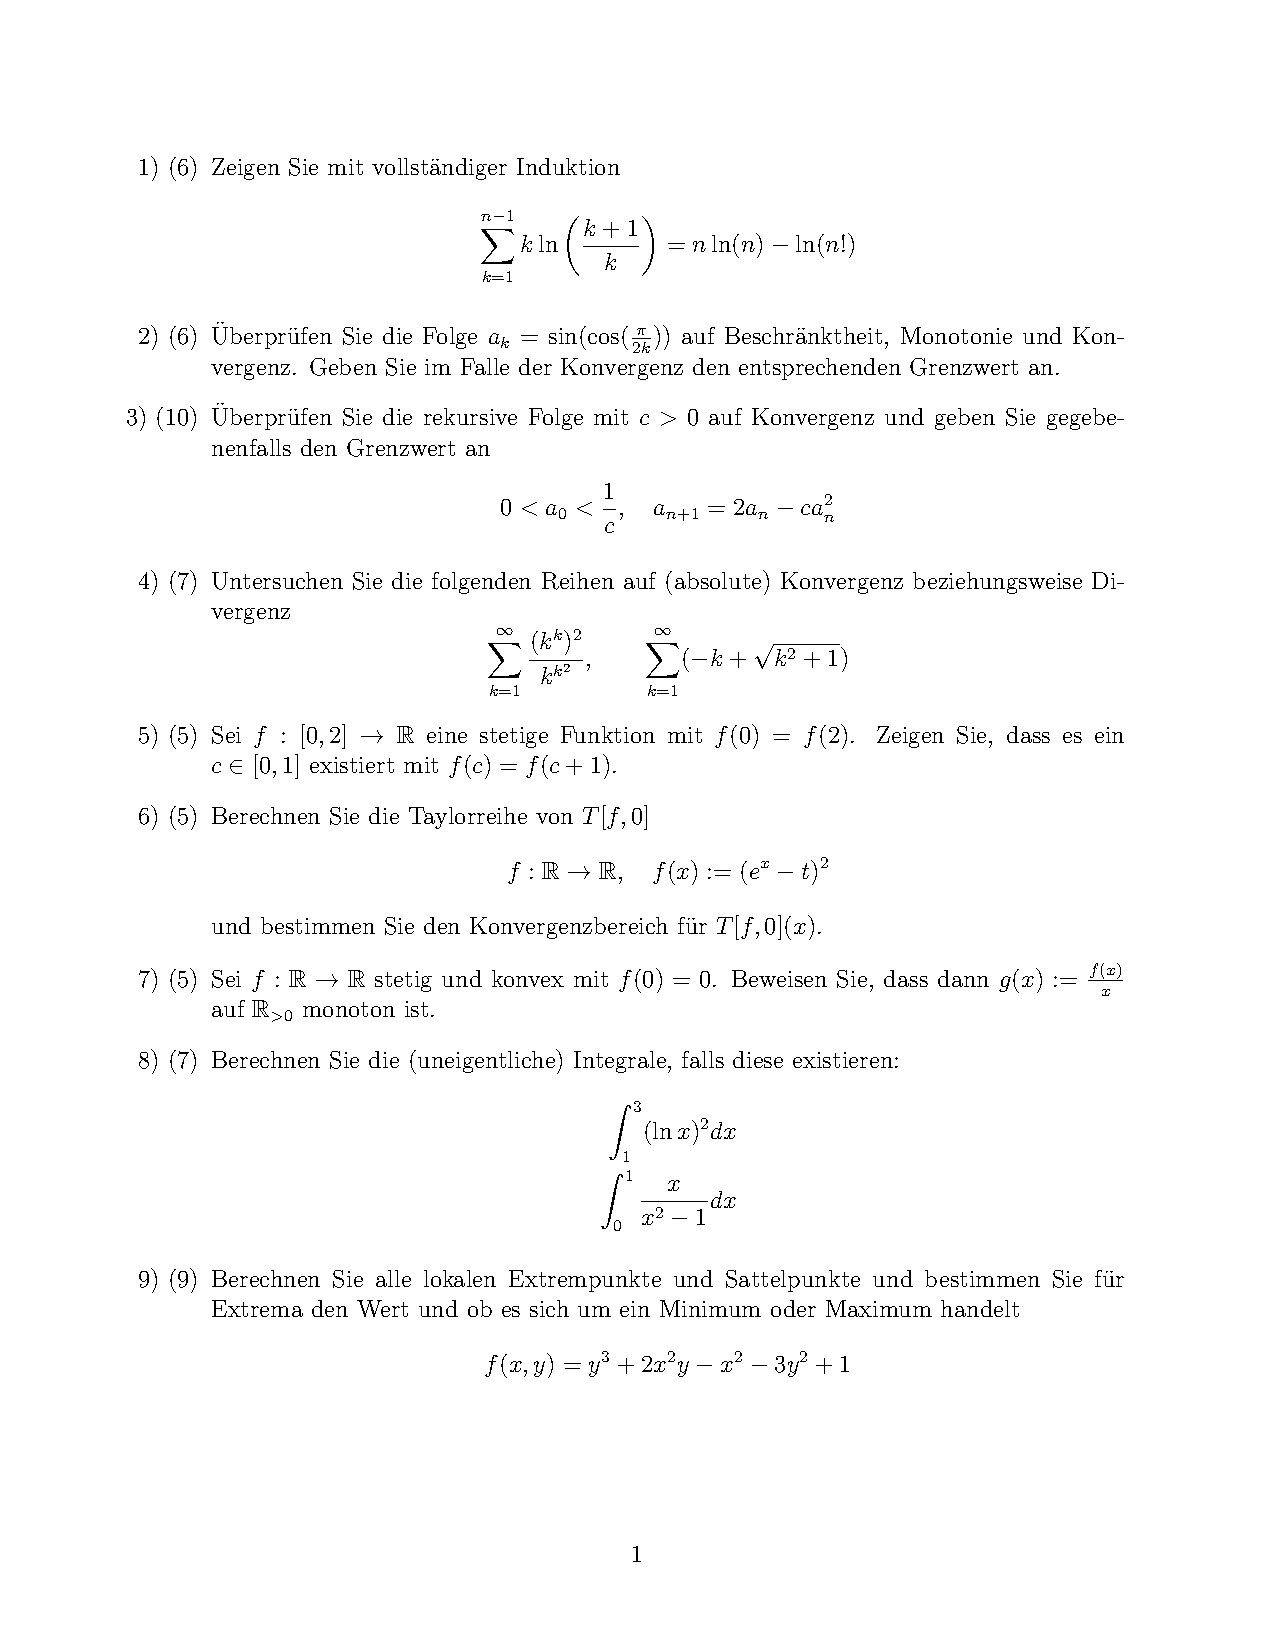
\includegraphics[page=1]{2022.07.05/Probeklausur2.pdf}    

\subsection{Musterlösungsweg Alexander Frank}
\subsubsection{Aufgabe 1}
Induktionsanfang: $(n = 1)$\\
Induktionsvoraussetzung: $\exists n \in \N: A(n)$\\
Induktionsschritt: $(n \rightarrow n+1)$
\begin{align*}
    n\ln(\frac{n+1}{n}) + \sum^{n - 1} ...\\
    \overset{I.V.}{=} n \ln(\frac{n+1}{n}) + n \ln n - \ln (n!)
\end{align*}
Logarithmenregeln
\begin{align*}
    n\cdot \ln(n +1) - \ln(n!)
\end{align*}
+ $0$-Addition
\begin{align*}
    n \cdot \ln(n +1) - \ln (n!) \pm \ln(n+1)
\end{align*}
\subsubsection{Aufgabe 2}
\begin{align*}
    a_k = \sin(\cos(\frac{\pi}{24}))
\end{align*}
\begin{enumerate}[label=\roman*)]
    \item Beschränktheit:$\sin(y_K) \in [-1, 1]$
    \item Monotonie: $z_k = \frac{\pi}{2k} \in [0, \frac{\pi}{2}]$ monoton fallend\\
    $y_k = \cos(z_k)$ monoton steigend\\
    $a_k = \sin(y_k)$ monoton steigend
    \item Konvergenz: Beschränkt + Monoton $\Ra$ Konvergent
    \item Grenzwert: Stetigkeit
    \begin{align*}
        \lim_{n \rightarrow \infty} \sin(\cos(\frac{\pi}{2k})) = \sin(\cos(0)) = \sin(1)
    \end{align*}
\end{enumerate}
\subsubsection{Aufgabe 3}
\begin{enumerate}[label=\roman*)]
    \item Beschränktheit: 
    \begin{align*}
        a_0 \in (0, \frac{1}{c}), a_1 \in (0, \frac{1}{c})
    \end{align*}
    Induktiv zeigen $0 < a_{n} < \frac{1}{c} \forall n \in \N_0$
    \begin{align*}
        0 &< 2a_n - ca_n^2 < \frac{1}{c} &\Leftrightarrow\\
        0 &< \frac{2}{c} a_n - a_n^2 < \frac{1}{c^2} &\Leftrightarrow\\
        0 &< \frac{1}{c^2} - \frac{1}{c^2} + \frac{2}{c}a_n + - a_n ^2 < \frac{1}{c^2} &\Leftrightarrow\\
        0 &< \frac{1}{c^2} - (\frac{1}{c} - a_n)^2 < \frac{1}{c^2}
    \end{align*}
    \item Monotonie: 
    $a_{n+1} \geq a_n \ \forall n \in \N$
    \item Konvergenz: $a = 2a - ca^2$
    \begin{align*}
        a &= 2a - ca^2\\
        ca^2 - a &= 0\\
        ca(a - \frac{1}{c}) &= 0
    \end{align*}
\end{enumerate}
\subsubsection{Aufgabe 4}
a)$\sum_{k=1}^\infty \frac{(k^k)^2}{k^{k^2}}$
\begin{align*}
     \sum_{k=1}^\infty \frac{(k^k)^2}{k^{k^2}} &= \sum_{k=1}^\infty \frac{k^{2k}}{k^{k^2}}
\end{align*}
\begin{align*}
    \lim_{n \rightarrow \infty} \frac{k^2}{k^k} = \frac{1}{k^{k - 2}} \overset{n \rightarrow \infty}{\rightarrow} 0
\end{align*}
b) $\sum_{k=1}^\infty (-k + \sqrt{k^2 + 1})$
\begin{align*}
    \rightarrow \text{3. Binomische Erweiterung} 1- \text{Multiplikation}
\end{align*}
3. Binomische Erweiterung: $\sum (b -  \sqrt{a}) \frac{(b + \sqrt{a})}{b + \sqrt{a}}$
\begin{align*}
    \sum_{k=1}^\infty (-k + \sqrt{k^2 + 1}) &= \sum_{k=1}^\infty \frac{1}{k + \sqrt{k^2 + 1}}
\end{align*}
$\rightarrow $ Minorantenkriterium 
\begin{align*}
    \sum_{k=1}^\infty \frac{1}{k + \sqrt{k^2 + 1}} > \sum_{k=1}^\infty \frac{1}{k + \sqrt{k^2  + k^2}} = \frac{1}{1 + \sqrt{2}} \sum_{k=1}^\infty \frac{1}{k}
\end{align*}
\subsubsection{Aufgabe 5}
Zwischenwertsatz
\begin{align*}
    g(x) := f(x) - f(x + 1)
\end{align*}
$ [0, 1]$ stetig\\
\begin{enumerate}
    \item $f(1) > f(0) $
    \item $f(1) = f(0) $
    \item $f(1) < f(0) $
\end{enumerate}
ZWS $A(x) = B(x) \Rightarrow 0 = A(x) - B(x) $
\subsubsection{Aufgabe 6}
Ableitungen bestimmen\\
$f^{(k)}$ bestimmen: Induktion\\
Tylorreihe bestimmen\\
\begin{align*}
    f(x) = (e^x - t)^2 = e^{2x} - 2te^x +t^2\\
    f'(x) = 2e^{2x} - 2te^x\\
    f''(x) = 2^2 e^{2x} - 2te^x
\end{align*}
\begin{align*}
    \sum_{k = 0}^\infty \frac{f^{(k)}(x_0)}{k!} x^k &= (1 - 2t + t^2) + \sum_{k=1}^\infty ...\\
    &= (1 - 2t + t^2) + \sum_{k = 1}^\infty  \frac{2k - 2t}{k!} x^k
 \end{align*}
\subsubsection{Aufgabe 7}
f stetig, konvex, $f(0) = 0$, $g(x) = \frac{f(x)}{x}$ monoton!\\
\begin{align*}
    f(\lambda x + ( 1 - \lambda) y) \leq \lambda f(x) + (1 - \lambda) f(y)
\end{align*}
$x = 0, y > 0$
\subsubsection{Aufgabe 8}
a)\\
$\rightarrow$ Partielle Integration\\
$\rightarrow$ Stammfunktion $\ln x$\\
b)\\
$\rightarrow$ Substitutionelle Integration
$\rightarrow$ oder kürzen
$\rightarrow$ $1 = \lim_{c \rightarrow 1} c$
\subsubsection{Aufgabe 9}
$f(x, y) = y^3 + 2x^2y + x^2 - 3y^2 + 1$
\begin{enumerate}
    \item Begründe Differenzierbar
    \item Gradient bilden $\Delta f(x, y) = \binom{\delta x f}{\delta y f}$
    \item $\Delta^2 f = Hf = \left(\begin{array}{cc}
        \delta xx &  \delta xy \\
        yx & \delta yy
    \end{array}\right)$
    \item Löse $\delta x f= 0 \land \delta y f = 0$
    (Hier 4 Lösungen)
    \item Punkte in $\sigma^2 f(x_0, y_0)$ $ab - c^2$
\end{enumerate}
\end{document}